\section{Irreversible Perturbation}

For the reasons explained in the previous section, ${\varkappa}_{\rm A \rightarrow \partial AB }$ is rarely independent of time in real systems.
Let us discuss the irreversible reaction (\ref{eq:A-to-B}) generalised to phase space.
Let the configuration space be divided into two boxes, A and B.
Let all the microstates of the system be in equilibrium.
At time $t=0$ we irreversibly disturb the equilibrium, so that the population of states in box B is zero:
\begin{equation}
\label{eq:start-irrev}
\begin{split}
\rho ({\bf p},{\bf q} , 0 ) \equiv 0 ~~~ \forall ({\bf p},{\bf q} ) \notin A ~ ,
\\
\rho ({\bf p},{\bf q} , 0 ) \equiv 1 ~~~ \forall ({\bf p},{\bf q} ) \in A ~ .
\end{split}
\end{equation}
From time $t=0$ we let the system evolve in a way such that no trajectory can leave box B (Figure \ref{fig:irrev-trajs}).

\begin{figure}[h]
\centering
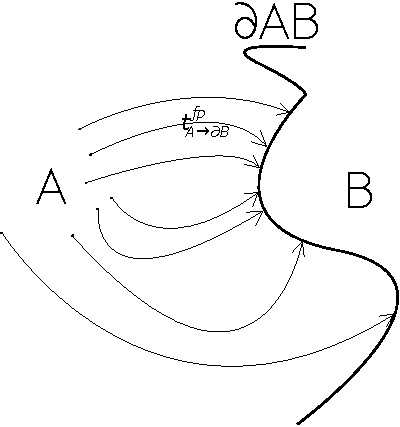
\includegraphics[height=6cm]{Images/diagAtoB.pdf}
\caption[Trajectories ending at the dividing surface.]{Illustration of the reactive trajectories. Each trajectory starts at a phase state in A and ends at the boundary of box B. The distribution of trajectories entering B (normalised flux $F_{\rm A\rightarrow \partial AB}$) is equal to the distribution of first passage times.}
\label{fig:irrev-trajs}
\end{figure}

Let us assume that box A has some internal barriers and that the dividing surface between A and B is rough.
The $P(t)$ decay will be steeper at low time values because of surface roughness and slower at high time values because of internal barriers.
The rate constant describing the dynamics during the whole process can be obtained by fitting the evolution to an exponential function using least squares, leading to the equation:
\begin{equation}
\label{eq:lsq}
\frac{\partial}{\partial k_{\rm A \rightarrow \partial B }} \int_0^{\infty} \!\! \left( P(t) - e^{- k_{\rm A \rightarrow \partial B } t } \right)^2 ~ {\rm d}t = 0 ~,
\end{equation}
which can be solved numerically.
The reactive flux method in this case leads to:
\begin{equation}
\label{eq:eq-flux-nonexp}
k^{TST}_{\rm A \rightarrow \partial B } = \frac{F(0)}{P(0)} ~,
\end{equation}
which is generally different from the expression (\ref{eq:lsq}) for the rate constant the best describes the process.

Although the reciprocal of the MFPT is not generally equal to $k$ in equation (\ref{eq:lsq}), it can be a good approximation of the rate constant.
First, the MFPT involves information about $P(t)$ for all times $t$.
Second, the MFPT often identified with the ``waiting time" is explicitly required by some methods for dynamical simulation, including the kinetic Monte Carlo\cite{Bortz1975, Gillespie1976, Fichthorn1991} and DPS approach.
The MFPT is the ensemble average of the time it takes for the equilibrium distribution to pass through the dividing surface:
\begin{equation}
\label{eq:mfpt-def}
{\rm MFPT_{A \rightarrow \partial AB}} = \frac{\displaystyle{\int t^{fp}_{\rm A \rightarrow \partial AB}({\bf p} ,{\bf q}) ~ H({\bf p},{\bf q}, {\rm A}) ~ {\rm d} {\bf p} {\rm d} {\bf q}}}
{\displaystyle{\int \! H({\bf p},{\bf q}, {\rm A}) ~ {\rm d} {\bf p} {\rm d} {\bf q}}} ~,
\end{equation}
where $H({\bf p},{\bf q},{\rm A})$ is 1 if $({\bf p},{\bf q})$ is in A and 0 otherwise.
Let us now compare how rate constants defined as the equilibrium flux and the reciprocal value of the MFPT fit a non-exponential $P(t)$.
A good test function is
\begin{equation}
\label{eq:test-ftn}
P(t) = c_1 e^{-c_2 t} + (1-c_1) e^{- t} ~.
\end{equation}
Low values of parameter $c_1$ represent small deviations from a strictly exponential distribution.
High values of the parameter $c_2$ represent deviations resulting from surface roughness, while low values model the effect of internal barriers.
From figure \ref{fig:diagram-k} it is obvious that the rate constant definition based on equilibrium flux fails to describe the long-time dynamics even for small deviations.
The MFPT rate constant can be used for very rough surfaces and very high internal barriers (values of $c_2$ very small or very large, respectively) provided the proportion of the affected phase space ($c_1$) is small.

\begin{figure}[h]
\centering
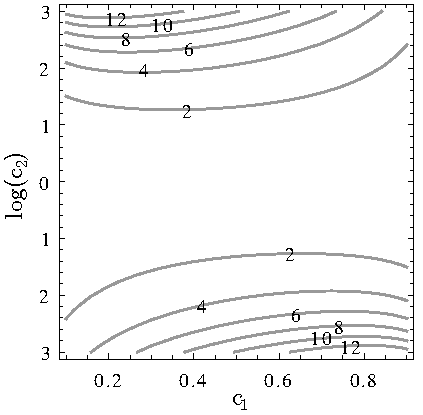
\includegraphics[height=7cm]{Images/derivk.pdf}
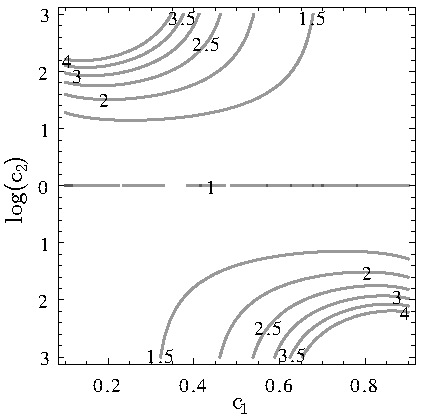
\includegraphics[height=7cm]{Images/intk.pdf}
\caption[Performance of TST and MFPT rate constants.]{Quality of the description of long-time dynamics using TST (left) and MFPT (right) rate constants as a function of $c_1$ and $\log(c_2)$ from (\ref{eq:test-ftn}) given as the ratio of the TST (MFPT) rate constants to the rate constant obtained analytically as the solution to (\ref{eq:lsq}). Isosurface contours represent values of $k$ 1.5 to 4 times higher for the MFPT and 2 to 12 times higher for TST. The MFPT rate constant generally lies much closer to the best value.}
\label{fig:diagram-k}
\end{figure}


\section{A Reversible Reaction}

Now let us consider a reversible reaction $\rm A \rightleftharpoons B$.
At time $t=0$ we irreversibly disturb the equilibrium, so that the population of states is distributed according to equation (\ref{eq:start-irrev}).
Fitting the evolution (\ref{eq:A-to-B-and-back-a-of-t}) leads to rate constants that are not generally consistent with the exit MFPT rate constants derived in the previous section.
It is obvious from figure \ref{fig:maze} that the change of an infinitesimally small part of box A does not affect the equilibrium between box A and B but it can affect the MFPT$_{\rm A \rightarrow \partial AB}$.
Therefore, the rate constants calculated from the exit MFPT will not have the property (\ref{eq:eq-const}).

\begin{figure}[h]
\centering
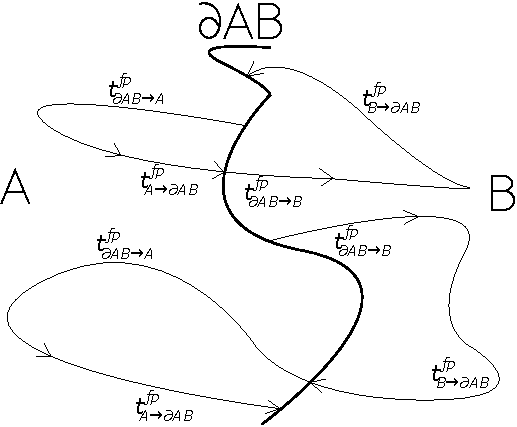
\includegraphics[height=6cm]{Images/diagAtoBtoA.pdf}
\caption[Reactive trajectories for a reversible transition.]{Illustration of reactive trajectories. Each trajectory starting at ${\rm \partial AB}$ going through box A returning to ${\rm \partial AB}$ can be divided into penetration ${\rm \partial AB \rightarrow A}$ and exit ${\rm A \rightarrow \partial AB}$ trajectories.}
\label{fig:rev-trajs}
\end{figure}

The inconsistency originates in the neglect of the penetration time in the calculation of MFPT$_{\rm A \rightarrow B}$.
The whole transition from box A in equilibrium to B in equilibrium can be divided into two consecutive processes.
First, trajectories must leave box A by reaching the boundary ${\rm \partial AB}$.
Then, they propagate from ${\rm \partial AB}$ to B, such that their end points are distributed according to equilibrium probability in B.
All trajectories ${\rm \partial AB \rightarrow A \rightarrow \partial AB}$ can be therefore divided into exit and penetration trajectories.
If the phase points in A are in equilibrium with other phase points lying on the same trajectory in A throughout the whole process, the ratio of leaving to penetration times is given by the ratio of the corresponding equilibrium fluxes:
\begin{equation}
\label{eq:leave-penetrate}
\frac{F_{\rm A \rightarrow B}(t)}{P_{\rm A}(t)} ~ {\rm MFPT_{\rm A \rightarrow \partial AB}}  
= \frac{F_{\rm B \rightarrow A}(t)}{P_{\rm B}(t)} ~ {\rm MFPT_{\rm \partial AB \rightarrow A}} ~.
\end{equation}
The rate constant calculated as 
\begin{equation}
\label{eq:corrected}
k_{\rm A \rightarrow B} = \frac{1}{\rm MFPT_{\rm A \rightarrow B}} = 
\frac{f_{\rm AB} + f_{\rm BA}}{f_{\rm AB} \left( \rm MFPT_{\rm \partial AB \rightarrow A \rightarrow \partial AB}  + MFPT_{\rm \partial AB \rightarrow B \rightarrow \partial AB} \right) }
~,
\end{equation}
where $f_{\rm ij} = F_{\rm i \rightarrow j}(t) / P_{\rm i}(t)$, gives the correct equilibrium distribution.
The reactive flux approach can give the correct equilibrium properties but the MFPT's have to be used for calculating the rate constants. 


